% Define Width and Height
\def\rectWidth{6.6in}
\def\rectHeight{.5in}

% Goes from -0.5 (INFO) to +0.5 (CRITICAL)
\def\score{0.3}

\pgfdeclarehorizontalshading{grad1}{2in}{
    color(0.0cm)=(infoBlue);
    color(0.55cm)=(lowGreen);
    color(0.865cm)=(mediumOrange);
    color(1.5cm)=(highRed);
    color(1.8cm)=(criticalPurple);
    color(2cm)=(criticalPurple)
}


\begin{tikzpicture}[remember picture,overlay,every node/.style={inner sep=0,outer sep=0}]
    % Draw Gradient
    \fill [shading=grad1,shading angle=0, draw=black, line width=1pt] rectangle +(\rectWidth,\rectHeight);

    % Draw Labels
    \node (infoBlue) [node font=\Large, color=infoBlue, xshift=.35in, yshift=-.7in] {\textbf{\LARGE Info}};
    \node (lowGreen) [right of=infoBlue, node distance=1.4in, font=\Large, color=lowGreen] {\textbf{\LARGE Low}};
    \node (mediumOrange) [right of=lowGreen, node distance=1.5in, font=\Large, color=mediumOrange] {\textbf{\LARGE Medium}};
    \node (highRed) [right of=mediumOrange, node distance=1.5in, font=\Large, color=highRed] {\textbf{\LARGE High}};
    \node (criticalPurple) [right of=highRed, node distance=1.4in, font=\Large, color=criticalPurple] {\textbf{\LARGE Critical}};

    % Draw Triangles
        % Define the dimensions of the triangles
    \def\triangleHeight{0.4*\rectHeight}
    \def\triangleWidth{1.0*\rectHeight}  % Adjust this value to squash the triangle
    
    % Define the vertical shift for the triangles
    \def\shiftUp{0.2*\rectHeight}
    \def\shiftDown{0.8*\rectHeight}
    
    % Define the horizontal shift for the triangles
    \def\shiftLeft{\score*\rectWidth}
    
    \fill [shading=grad1,shading angle=0, draw=black, line width=1pt] rectangle +(\rectWidth,\rectHeight);
    
    \draw[black, fill=black] (\rectWidth/2+\shiftLeft,-\rectHeight+\shiftDown) -- ++(-\triangleWidth/2,-\triangleHeight) -- ++(\triangleWidth,0) -- cycle;
    
    \draw[black, fill=black] (\rectWidth/2+\shiftLeft,\rectHeight+\shiftUp) -- ++(-\triangleWidth/2,\triangleHeight) -- ++(\triangleWidth,0) -- cycle;
\end{tikzpicture}\vspace{2cm}

\newpage

\textbf{RATIONALE:} Overall, \team was impressed by the network architecture and security measures put in place by \client to protect company machines and user data. There were clear efforts to prevent the usage of malware on the machines and there were several critical vulnerabilities addressed, which mitigated the ability of \team to breach the systems. The majority of the Windows domain and high-privileged users were secure and guarded against privilege escalation. Docker containers assessed were securely configured to prevent escapes to the host operating system, and web services securely sanitized that stopped most injection attacks (such as SQL and XSS). However, \team discovered multiple vulnerabilities leading to exposure of sensitive information and concluded that \client still faces a \textbf{\textcolor{highRed}{high}} risk of compromise. 

On Windows, there are several vulnerabilities that allowed for access to the machines. Due to these vulnerabilities, \team was able to gain access to high-privilege accounts on a server and low-privilege access on the remaining servers.

On \clientP web services, there were several vulnerabilities that enabled \team to impersonate and take actions on behalf of other users, delete users, and modify critical databases controlling ship operations - thus putting \clientP system, clients, and reputation at risk.

\team posits that the major vulnerabilities found on \clientP Windows machines and web applications are in violation of the three key tenets of the CIA Triad, which are confidentiality, integrity, and availability. The discovered vulnerabilities could expose confidential user data, allow attackers to compromise the integrity of \client systems, and decrease system availability. Thus, assigning \client a high compromise risk was appropriate.

%\includeFigure{images/CIATriad.png}{CIA Triad}

%\newpage


% \begin{figure}[h!]
%         \centering
%         \begin{adjustbox}{cframe={\currentFindingColor} \imageBorderWidth}
%             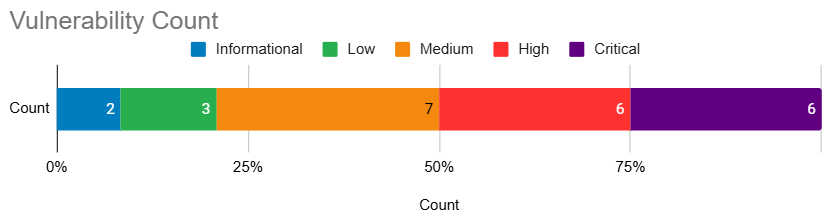
\includegraphics[width=4in]{images/plot-vulnerability-count}  
%         \end{adjustbox}
%         \captionsetup{labelfont={color=\currentFindingColor},textfont={color=\currentFindingColor}}
%         \caption{Vulnerability Count by Severity}
%         \label{fig:vulnsBySeverity}
%     \end{figure}  


% \includeFigure{images/ufsit.jpg}{Vulnerability Count by Category}{fig:vulnsByCategory}


% \includeFigure{images/ufsit}{Remediations}{fig:remchart}
